We now turn to the dependence structure between the French and German day-ahead electricity markets. After studying the marginal temporal dynamics and the distributional behavior of extreme observations, our goal is to characterize the joint dependence between the two markets in a way that goes beyond linear correlation.

The copula framework is particularly well suited to this task because it separates marginal behavior from the dependence structure. In our setting, this allows us to study whether French and German prices become jointly extreme during stress episodes, and whether this dependence is symmetric or concentrated in a specific tail.

\subsection{Variables and pseudo-observations}

To reduce the impact of deterministic seasonal effects, we work with de-seasonalized hourly price variations for France and Germany, denoted by \(X_t\) and \(Y_t\). These transformed variables are intended to capture the short-run residual market fluctuations after removing regular hourly and weekly patterns.

Following the copula methodology, we construct pseudo-observations
\[
\hat U_t = \hat F_X(X_t), \qquad \hat V_t = \hat F_Y(Y_t),
\]
where \(\hat F_X\) and \(\hat F_Y\) are the empirical marginal distribution functions. This step maps the original observations to the unit square and isolates the dependence structure from the marginal scales.

Figure~\ref{fig:copula_scatter} displays both the scatter plot of the transformed French and German variations and the corresponding pseudo-observations. The raw scatter plot already suggests a positive dependence, while the pseudo-observation plot reveals that the dependence is not purely elliptical and may be stronger in the upper tail.

\begin{figure}[H]
    \centering
    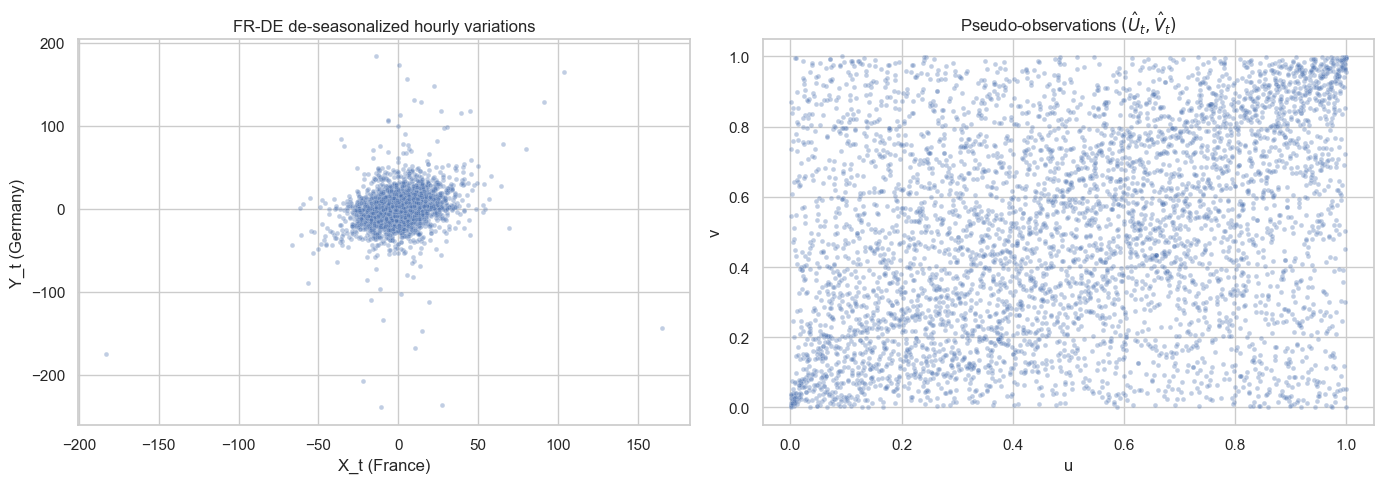
\includegraphics[width=0.96\textwidth]{figures/copula_scatter.png}
    \caption{Left: scatter plot of de-seasonalized hourly price variations in France and Germany. Right: pseudo-observations \((\hat U_t, \hat V_t)\) used for copula estimation.}
    \label{fig:copula_scatter}
\end{figure}

\subsection{Rank-based dependence measures}

We begin with nonparametric rank-based indicators. On the full sample, the Kendall coefficient is estimated at
\[
\hat\tau = 0.2177,
\]
while the Spearman coefficient is
\[
\hat\rho = 0.3062.
\]

These values indicate a positive but moderate dependence between the two markets. The two price series are clearly linked, but not in a way that would suggest near-deterministic co-movement. This makes the copula approach relevant: there is enough dependence to be modeled, but enough flexibility left to distinguish between alternative dependence structures.

\subsection{Parametric copula families}

We estimate three parametric copula families that were studied in the course: the Gaussian copula, the Gumbel copula, and the Clayton copula. The Gaussian copula is a natural benchmark but does not exhibit tail dependence. By contrast, the Gumbel copula captures upper-tail dependence, whereas the Clayton copula captures lower-tail dependence. This distinction is especially relevant for electricity prices, where the economic interpretation of very high prices and very low or negative prices is quite different.

For each family, we consider two estimation strategies: inversion of Kendall's tau and maximum likelihood based on the pseudo-observations. We then compare the fitted models through their log-likelihood, AIC, BIC, and implied tail-dependence coefficients.

Table~\ref{tab:copula_full} reports the results on the full sample.

\begin{table}[H]
\centering
\caption{Copula estimation results on the full sample.}
\label{tab:copula_full}
\begin{tabular}{lcccccccc}
\toprule
Family & \(\hat\tau\) & \(\hat\rho\) & Param. (tau) & Param. (MLE) & \(\ell_{\text{tau}}\) & \(\ell_{\text{MLE}}\) & \(\lambda_l\) & \(\lambda_u\) \\
\midrule
Gaussian & 0.2177 & 0.3062 & 0.3353 & 0.3113 & 294.6647 & 297.0064 & 0.0000 & 0.0000 \\
Gumbel   & 0.2177 & 0.3062 & 1.2783 & 1.2773 & 392.1663 & 392.1692 & 0.0000 & 0.2794 \\
Clayton  & 0.2177 & 0.3062 & 0.5566 & 0.3938 & 215.6555 & 245.2915 & 0.1720 & 0.0000 \\
\bottomrule
\end{tabular}
\end{table}

The ranking is unambiguous on the full sample: the Gumbel copula clearly dominates the Gaussian and Clayton alternatives. It yields the highest log-likelihood and the best information criteria, which indicates that the dependence between the two markets is better described by an asymmetric structure with upper-tail dependence than by a symmetric Gaussian benchmark or a lower-tail-dependent Clayton copula.

This result is economically meaningful. It suggests that the strongest common dependence between the French and German markets does not occur primarily during jointly very low prices, but rather during jointly high price episodes. In other words, the two markets appear especially connected when upward stress affects both systems at the same time.

\subsection{Calm versus stressed regimes}

To go beyond the average dependence structure, we split the sample into a calm regime and a stressed regime, based on large spread or volatility conditions. The purpose is not only to determine which copula performs best overall, but also to understand whether the form of dependence changes across market regimes.

Table~\ref{tab:copula_regimes} summarizes the corresponding estimates.

\begin{table}[H]
\centering
\caption{Copula estimation results by regime.}
\label{tab:copula_regimes}
\begin{tabular}{llcccccc}
\toprule
Regime & Family & \(\hat\tau\) & \(\hat\rho\) & Param. (MLE) & \(\ell_{\text{MLE}}\) & \(\lambda_l\) & \(\lambda_u\) \\
\midrule
Calm     & Gaussian & 0.2231 & 0.3168 & 0.3659 & 237.2648 & 0.0000 & 0.0000 \\
Calm     & Gumbel   & 0.2231 & 0.3168 & 1.3341 & 299.8596 & 0.0000 & 0.3187 \\
Calm     & Clayton  & 0.2231 & 0.3168 & 0.5021 & 195.2759 & 0.2514 & 0.0000 \\
Stressed & Gaussian & 0.2073 & 0.2888 & 0.2364 & 75.9999  & 0.0000 & 0.0000 \\
Stressed & Gumbel   & 0.2073 & 0.2888 & 1.1926 & 107.9107 & 0.0000 & 0.2118 \\
Stressed & Clayton  & 0.2073 & 0.2888 & 0.2633 & 67.7384  & 0.0719 & 0.0000 \\
\bottomrule
\end{tabular}
\end{table}

Several points emerge from this comparison. First, the Gumbel copula remains the best-performing family in both regimes, which makes the main conclusion robust. Second, the overall rank dependence is slightly stronger in the calm regime than in the stressed regime, as seen from both Kendall's tau and Spearman's rho. Third, upper-tail dependence remains present in both regimes, but is estimated to be larger in the calm regime than in the stressed one.

At first sight, the last point may seem surprising. One might expect stronger upper-tail dependence precisely during stressed periods. However, our stress partition captures high-volatility or large-spread situations more broadly, which may include heterogeneous episodes in which the two markets do not always move to the same extreme at the same time. In that sense, the stressed regime may contain more dispersion and more local asymmetries, even though it remains more turbulent.

\subsection{Empirical copula diagnostics and tail concentration}

Figure~\ref{fig:copula_heatmap} shows the empirical copula heatmap, while Figure~\ref{fig:copula_contours} presents the fitted contours for the three parametric families. These figures are useful because they complement the likelihood-based comparison with a direct visual representation of the dependence structure.

\begin{figure}[H]
    \centering
    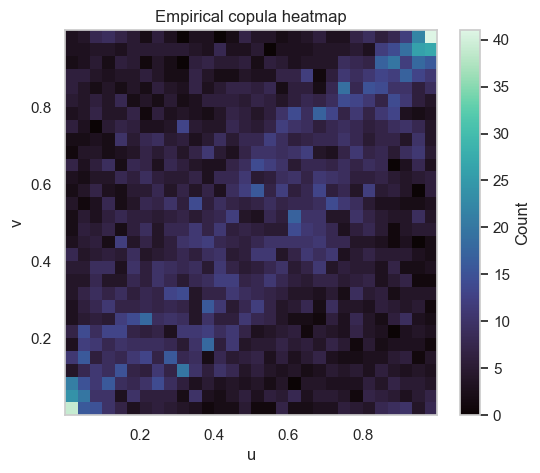
\includegraphics[width=0.58\textwidth]{figures/copula_heatmap.png}
    \caption{Empirical copula heatmap based on the pseudo-observations.}
    \label{fig:copula_heatmap}
\end{figure}

\begin{figure}[H]
    \centering
    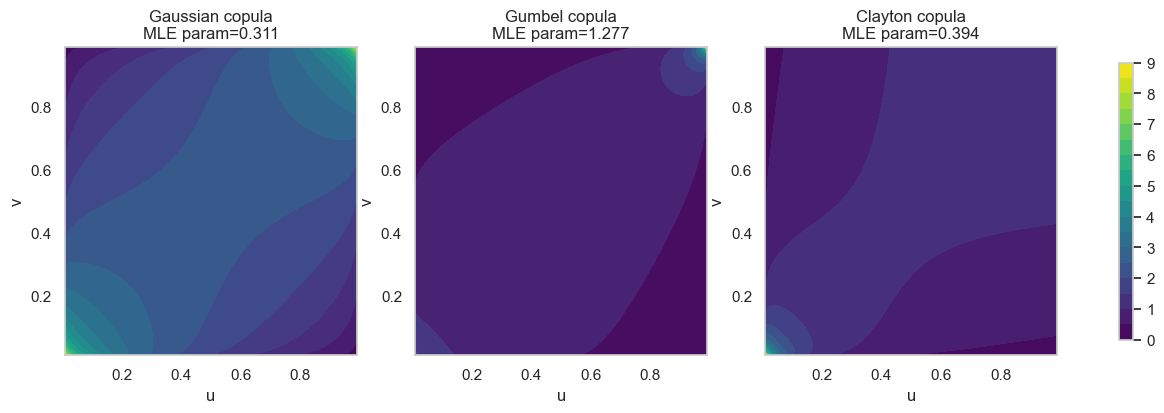
\includegraphics[width=\textwidth]{figures/copula_contour.png}
    \caption{Fitted copula contours for the Gaussian, Gumbel, and Clayton models.}
    \label{fig:copula_contours}
\end{figure}

We also examine empirical tail concentration functions in order to compare the lower and upper corners of the unit square. The lower-tail concentration decreases slowly and then appears to converge to zero for very small values of \(q\), which is not consistent with a very strong lower-tail dependence. By contrast, the upper-tail concentration is more structured: on the full sample it remains clearly positive, while in the stressed regime it becomes more irregular and even increases at very small values of \(q\). Although the smallest-\(q\) region must be interpreted cautiously because of limited sample size, this pattern is coherent with the dominance of the Gumbel family.

\begin{figure}[H]
    \centering
    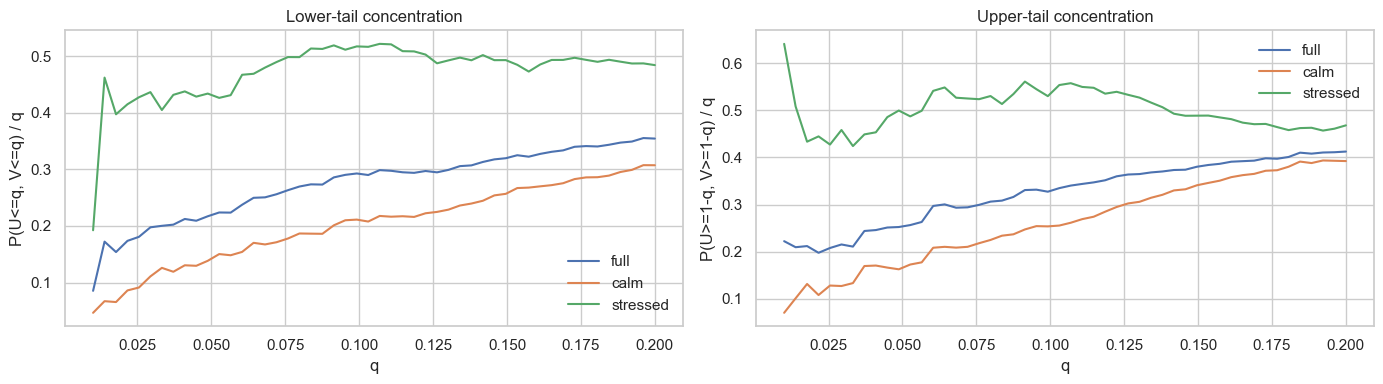
\includegraphics[width=\textwidth]{figures/copula_concentration.png}
    \caption{Empirical lower-tail and upper-tail concentration functions across regimes.}
    \label{fig:tail_concentration}
\end{figure}

\subsection{Interpretation}

Overall, the copula analysis shows that the dependence between French and German day-ahead prices cannot be reduced to average linear co-movement. The best-fitting copula is consistently the Gumbel copula, which points to an asymmetric dependence structure with upper-tail dependence. In economic terms, this means that the most informative joint behavior appears during common upward price stress, rather than during jointly very low or negative prices.

This conclusion complements the previous sections of the report. Once the marginal time-series dynamics have been accounted for, and once rare events have been identified through the extreme-value analysis, the copula framework reveals that dependence itself becomes more informative in the upper tail. This motivates the final step of our study: if extreme events occur jointly across markets, do they also cluster in time? This is the question addressed by the Hawkes-process analysis.